% ****** Start of file apssamp.tex ******
%
%   This file is part of the APS files in the REVTeX 4.1 distribution.
%   Version 4.1r of REVTeX, August 2010
%
%   Copyright (c) 2009, 2010 The American Physical Society.
%
%   See the REVTeX 4 README file for restrictions and more information.
%
% TeX'ing this file requires that you have AMS-LaTeX 2.0 installed
% as well as the rest of the prerequisites for REVTeX 4.1
%
% See the REVTeX 4 README file
% It also requires running BibTeX. The commands are as follows:
%
%  1)  latex apssamp.tex
%  2)  bibtex apssamp
%  3)  latex apssamp.tex
%  4)  latex apssamp.tex
%
\documentclass[%
 % reprint,
%superscriptaddress,
%groupedaddress,
%unsortedaddress,
%runinaddress,
%frontmatterverbose,
preprint,
%showpacs,preprintnumbers,
%nofootinbib,
%nobibnotes,
%bibnotes,
 amsmath,amssymb,
 aps,
 prd
%pra,
%prb,
%rmp,
%prstab,
%prstper,
%floatfix,
]{revtex4-1}

\usepackage{graphicx}% Include figure files
\usepackage{dcolumn}% Align table columns on decimal point
\usepackage{bm}% bold math
%\usepackage{hyperref}% add hypertext capabilities
%\usepackage[mathlines]{lineno}% Enable numbering of text and display math
%\linenumbers\relax % Commence numbering lines

%\usepackage[showframe,%Uncomment any one of the following lines to test
%%scale=0.7, marginratio={1:1, 2:3}, ignoreall,% default settings
%%text={7in,10in},centering,
%%margin=1.5in,
%%total={6.5in,8.75in}, top=1.2in, left=0.9in, includefoot,
%%height=10in,a5paper,hmargin={3cm,0.8in},
%]{geometry}

\newcommand{\ii}{\mathrm i}


%%%%%%%%%%%%%%%%%%%%%%%%%%%%%%%%%
%%%%% Packages for draft only
%%%%%%%%%%%%%%%%%%%%%%%%%%%%%%%%%%

\usepackage[normalem]{ulem}
\usepackage{xcolor}
\usepackage{accents}


\begin{document}

%\preprint{APS/123-QED}

\title{Dispersion Relation Gaps and Neutrino Flavor Instabilities in Fast Modes}% Force line breaks with \\
%\thanks{A footnote to the article title}%

\author{Lei Ma}
 \altaffiliation[Also at ]{Physics Department, XYZ University.}%Lines break automatically or can be forced with \\
\author{Huaiyu Duan}%
 \email{Second.Author@institution.edu}
\affiliation{%
 Authors' institution and/or address\\
 This line break forced with \textbackslash\textbackslash
}%


\date{\today}% It is always \today, today,
             %  but any date may be explicitly specified

\begin{abstract}

ABSTRACT PLACEHOLDER


% \begin{description}
% \item[Usage]
% Secondary publications and information retrieval purposes.
% \item[PACS numbers]
% May be entered using the \verb+\pacs{#1}+ command.
% \item[Structure]
% You may use the \texttt{description} environment to structure your abstract;
% use the optional argument of the \verb+\item+ command to give the category of each item.
% \end{description}
\end{abstract}

% \pacs{Valid PACS appear here}% PACS, the Physics and Astronomy
                             % Classification Scheme.
%\keywords{Suggested keywords}%Use showkeys class option if keyword
                              %display desired
\maketitle

%\tableofcontents



\section{\label{sec-introduction}Introduction}

(Should talk about some very very basic backgrounds like the applications and why it is important.)


Neutrino flavor conversions in vacuum are described by linear Sch\"{o}dinger eqution where the vacuum Hamiltonian doesn't depend on the state of neutrino flavors. It leads to periodic oscillations in different flavors. However, neutrinos propagate in dense neutrino media demonstrate highly nonlinear flavor transformations due to forward scattering interactions where the Hamiltonian is determined by the flavor contents. This nonlinear Schr\"{o}dinger equation can result in instabilities in neutrino flavor conversions. To investigate the complicated behavior of such nonlinear flavor conversions, linear stability analysis has been introduced \cite{Banerjee2011a,Raffelt2013}. Recent study by I. Izaguirre, G. Raffelt, and I. Tamborra showed that the dispersion relation gaps of the linearized equation of motion tell us the linear stability of neutrino flavor conversions \cite{Izaguirre2016a}. We will prove that neutrino flavor conversion instabilities is not exactly mapped to gaps in dispersion relation in some cases. In Sec. \ref{sec-dr}, we review linear stability analysis and dispersion relation based on references \onlinecite{Raffelt2013} and \onlinecite{Izaguirre2016a}.

(Introduce what are we gonna do in other sections when the paper is finished.)



\section{\label{sec-dr}Dispersion Relation of Neutrino Flavor Conversion}

We consider two-flavor scenario ($\nu_{\mathrm e}$ and $\nu_{\mathrm x}$) of neutrino oscillations. We also assume that all neutrinos and antineutrinos are emitted as electron flavor. The flavor evolution of neutrino ensemble depends on flavor density matrices of neutrinos $\rho$ and antineutrinos $\bar\rho$ with energy $E$, direction of velocity $\hat{\mathbf v}$,
\begin{equation}
\ii (\partial_t + \mathbf v\cdot \mathbf{\nabla}) \rho = \left[H, \rho_n \right],
\label{eqn-liouville-eqn}
\end{equation}
where $H$ is the Hamiltonian for neutrino oscillations. In the context, Hamiltonian depends on three different contributions from vacuum oscillations $H_{\mathrm v}$, interactions with matter $H_{\mathrm m}$, and interactions with neutrinos themselves $H_{\nu\nu}$. In this work, we ignore vacuum and matter terms since the concentration is on fast neutrino oscillations, which would occur even without neutrino mass differences \cite{Chakraborty2016,Dasgupta2017}. In order to calculate the neutrino self-interaction term $H_{\nu\nu}$, the distribution of neutrinos (antineutrinos) $f_{\nu_{\mathrm e}(\bar \nu_{\mathrm e})}(\hat{\mathbf v}, E)$ and $f_{\nu_{\mathrm x}(\bar \nu_{\mathrm x})}(\hat{\mathbf v}, E)$ is required, where $E$ is the energy of neutrinos (antineutrinos). We have
\begin{equation}
H_{\nu\nu} = \sqrt{2} G_{\mathrm F} \iint \frac{\mathrm d \cos\theta' \mathrm d\phi'}{4\pi} v^\mu v'_\mu \int \frac{E'^2 \mathrm d E'}{2\pi^2} \left( (f_{\nu_{\mathrm e}}' - f_{\nu_{\mathrm x}}' )\rho' -  (f_{\bar\nu_{\mathrm e}}' - f_{\bar\nu_{\mathrm x}}' ) \bar\rho' \right),
\end{equation}
where $v^\mu = ( 1, \sin\theta\cos\phi, \sin\theta\sin\phi, \cos\theta )^{\mathrm T}$ is the four velocity of (anti)neutrinos in our spherical coordinate system. Without vacuum contribution, the equation of motion for antineutrinos has the same form \cite{Duan2010}.

We follow the same assumption in reference \onlinecite{Izaguirre2016a} that the the distribution of $\nu_x$ and $\bar\nu_x$ are the same, namely $ f_{\nu_{\mathrm x}}(\hat{\mathbf v},E)  - f_{\bar\nu_{\mathrm x}}(\hat{\mathbf v},E)=0$. In addition, we have the same definition of electron lepton number (ELN) of neutrinos travelling in direction $\hat{\mathbf v}$ \cite{Izaguirre2016a},
\begin{equation}
G(\hat{\mathbf v}) =  \sqrt{2}G_{\mathrm F} \int \frac{E'^2 \mathrm d E'}{2\pi^2} ( f_{\nu_{\mathrm e}}(\cos\theta',\phi',E')  - f_{\bar\nu_{\mathrm e}}(\cos\theta',\phi',E')  ).
\end{equation}
To perform linear stability analysis, we assume that the density matrix has the form
\begin{equation}
\rho = \bar \rho = \begin{pmatrix}
1 & \epsilon \\
\epsilon^* & 0
\end{pmatrix},
\end{equation}
where $\lvert \epsilon \rvert \ll 1$. As a result, the linearized equations of motion depends only on $G(\hat{\mathbf v})$ and $\hat{\mathbf v}$. We also assume that all neutrinos and antineutrinos undergo the same behavior in linear regime, $\epsilon = \tilde\epsilon e^{-\ii (\Omega t - \mathbf K\cdot \mathbf x)}$. Izaguirre, Raffelt, and Tamborra defined the polarization tensor \cite{Izaguirre2016a},
\begin{equation}
\Pi^\mu_{\phantom{\mu}\nu} = 1 + \int \frac{d\Omega}{4\pi} G(\theta,\phi) \frac{v^\mu v_\nu}{\omega- k \hat{\mathbf k}\cdot \hat{\mathbf v} },
\end{equation}
which defines the dispersion relation $\Pi^\mu_{\phantom{\mu}\nu} a^\nu = 0$, with $a^\nu = \int \frac{d\cos\theta' d\phi'}{4\pi} G(\hat{\mathbf v}') v^\nu \tilde\epsilon$. We find the nontrivial solutions by setting \cite{Izaguirre2016a}, 
\begin{equation}
\operatorname{det}\left( \Pi^\mu_{\phantom{\mu}\nu} \right) = 0.
\label{eqn-dr-determinant-equation}
\end{equation}


For simplicity, we consider axial symmetric neutrino emission so that Eq. \eqref{eqn-dr-determinant-equation} becomes
\begin{align}
&\det \left( \omega \mathrm{I} + \frac{1}{2}
\begin{pmatrix}
   I_0 & 0 & 0 & -I_1 \\
   0 & -\frac{1}{2} (I_0 - I_2) & 0 & 0 \\
   0 & 0 & -\frac{1}{2} (I_0 - I_2) & 0 \\
   I_1 & 0 & 0 & -I_2
\end{pmatrix}\right) \nonumber\\
&=0,
\label{eqn-det-polarization-tensor-axial}
\end{align}
where $\mathbf I$ is the rank 4 identity matrix and
\begin{equation}
   I_m =\int_{-1}^{1} d u G(u) \frac{u^m}{1 -  \left(\lvert k\rvert /\omega\right) u }.
\end{equation}
where we define $u=\cos\theta$. Eq. \eqref{eqn-det-polarization-tensor-axial} is equivalent to the result in reference \onlinecite{Raffelt2013}. $\lvert k \rvert /\omega$ is defined as the refractive index $n$ of the flavor wave. For spectrum $G(u)$ without zero values, the forbidden region is given by $1 -  \left(\lvert k\rvert /\omega\right) u\leq 0$. 

The dispersion relations can be categorized into two different types by symmetries. To incorporate azimuthal symmetry, we define solutions related to the first and second element of $a^\nu$ ($\nu=1,2$) to be multi-azimuthal angle (MAA) solutions since they are the only solutions that depend on azimuthal angle $\phi$. The other solutions which are related to $\nu=0,3$ are defined to be the multi-zenith angle (MZA) solutions. The MAA solution is related to symmetry breaking in azimuthal angle only, which is determined by
\begin{equation}
   \omega = \frac{1}{4}(I_0 - I_2).
   \label{eqn-maa}
\end{equation}
Similarly, the MZA solution is related to symmetry breaking in both azimuthal angle and zenith angle, which is
\begin{equation}
\omega = - \frac{1}{4} \left( I_0 - I_2 \pm \sqrt{ (I_0 + I_2 - 2 I_1) (I_0 + I_2 + 2 I_1) } \right).
\label{eqn-mza}
\end{equation}
We denote the solution associated with $+$ sign in Eq. \eqref{eqn-mza} as MZA+, while the solution assocated with $-$ sign as MZA-. The two solutions are connected to each other in dispersion relations. In general, it doesn't provide physical insights to distingush the two branches of solutions since they are simply two branches of the solution.

The solutions to Eq. \eqref{eqn-maa} and Eq. \eqref{eqn-mza} are dispersion relations $D(\omega,\mathbf k)$ for a chosen direction of $\hat{\mathbf k} = \hat{\mathbf z}$ with axial symmetric neutrino emission.



%%%%%%%%%%%%%%%%%
%% To BE Added
%%%%%%%%%%%%%%%%
% {\color{red}{\bf HAVE TO EXPLAIN THE IDEA OF GAP AND INSTABILITY HERE. Maybe Later?}}






\section{\label{sec-instabilities-and-gaps}Instabilities and Gaps}

In reference \onlinecite{Izaguirre2016a}, the authors relate gaps in dispersion relation to instabilities of neutrino oscillations. In this section, we review the idea of correspondence between gaps and instabilities first. Then we show that this relation is not a solid theory that can be generalized to all cases.

We continue the discussion of axial symmetric neutrino emissions but with discretized zenith angles $\theta$ thus discretized $u$. Hence the ELN is independent of azimuth angle $\phi$. For neutrino emission with $2$ zenith angles, the ELN spectrum is
\begin{equation}
G(u)= \sum_{i=1}^2 g_i \delta(u - u_i).
\end{equation}

The MAA solution becomes an equation of hypobola for $\omega$ and $k$, which has asymptotes $\omega = k u_i$ for $i=1,2$. Meanwhile, hyperbola equation has two solutions of $\omega$ ($k$) for any given real $k$ ($\omega$). The solutions are either real which indicates stable solutions or complex which indicates exponential growth or decrease in linear regime. On the other hand, non-existence of real solutions of $\omega$ ($k$) for given real $k$ ($\omega$) is equivalent to gap in dispersion relation. Thus the equivalence of gap and instabilities is guaranteed in neutrino emission with two-zenith-angle emission. Upper panels of Fig. \ref{fig-dr-db} is reproduction of left panels of Fig. 1 in reference \onlinecite{Izaguirre2016a}. The dispersion relation is shown as black lines. The real part $\omega_{\mathrm R}$ is shown as red solid lines. $\omega_{\mathrm R} \pm \omega_{\mathrm I}$ are shown are red dashed lines, where $\omega_{\mathrm I}$ is the imaginary part of $\omega$. 



\begin{figure}[!htb]
\minipage{0.49\textwidth}
  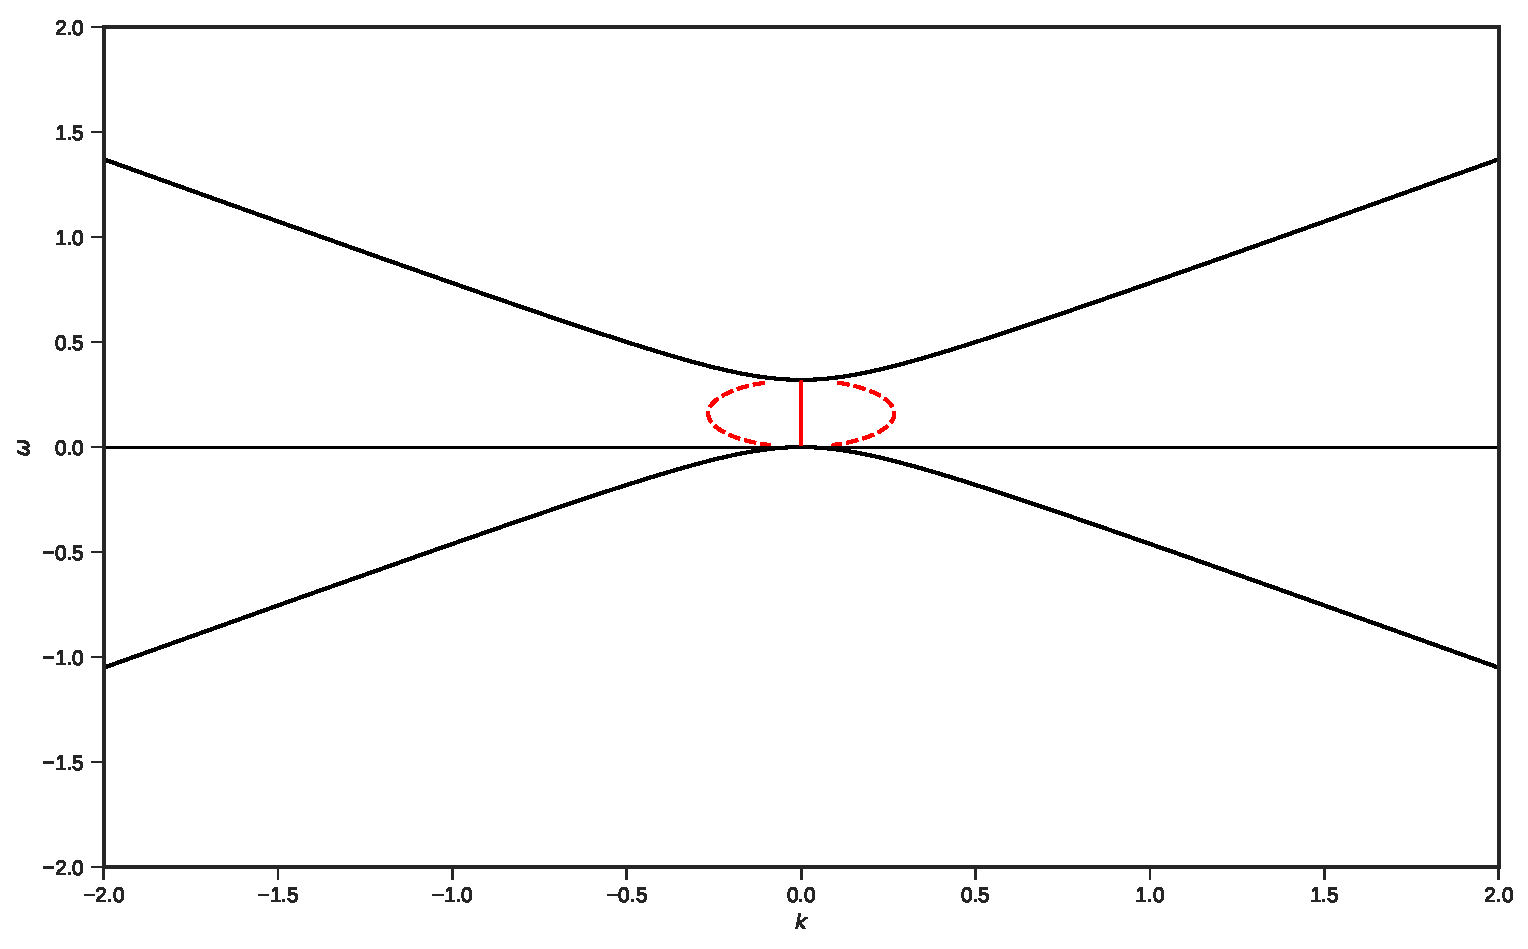
\includegraphics[width=\linewidth]{assets/spectDBWC1DRDBMAAPltBlob.pdf}
\endminipage\hfill
\minipage{0.49\textwidth}
  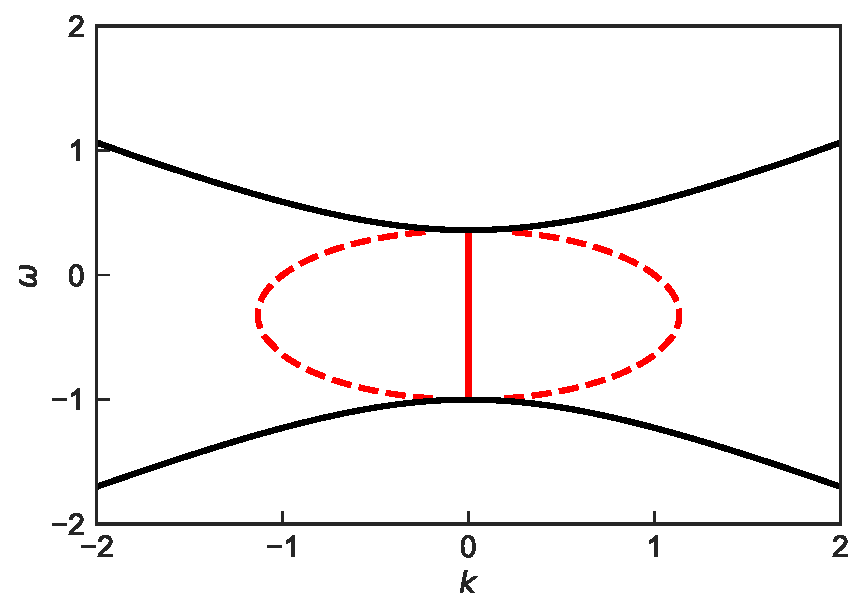
\includegraphics[width=\linewidth]{assets/spectDBWC1DRDBMZAPltBlob.pdf}
\endminipage\hfill
\newline
\minipage{0.49\textwidth}
  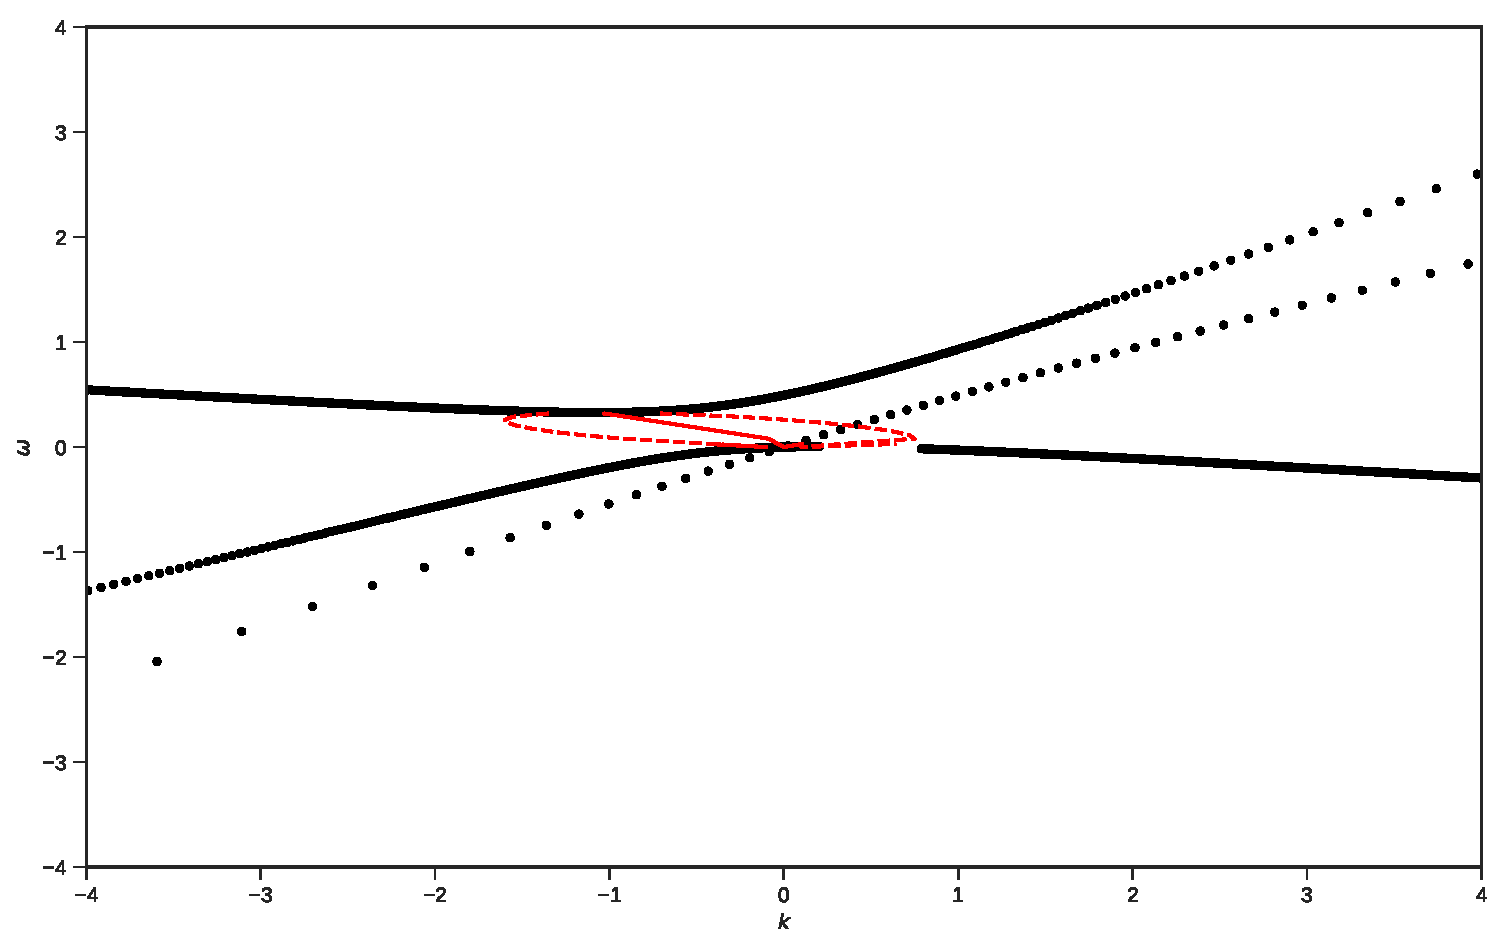
\includegraphics[width=\linewidth]{assets/spectDB3WC4DRDBMAAPltBlob.pdf}
\endminipage\hfill
\minipage{0.49\textwidth}
  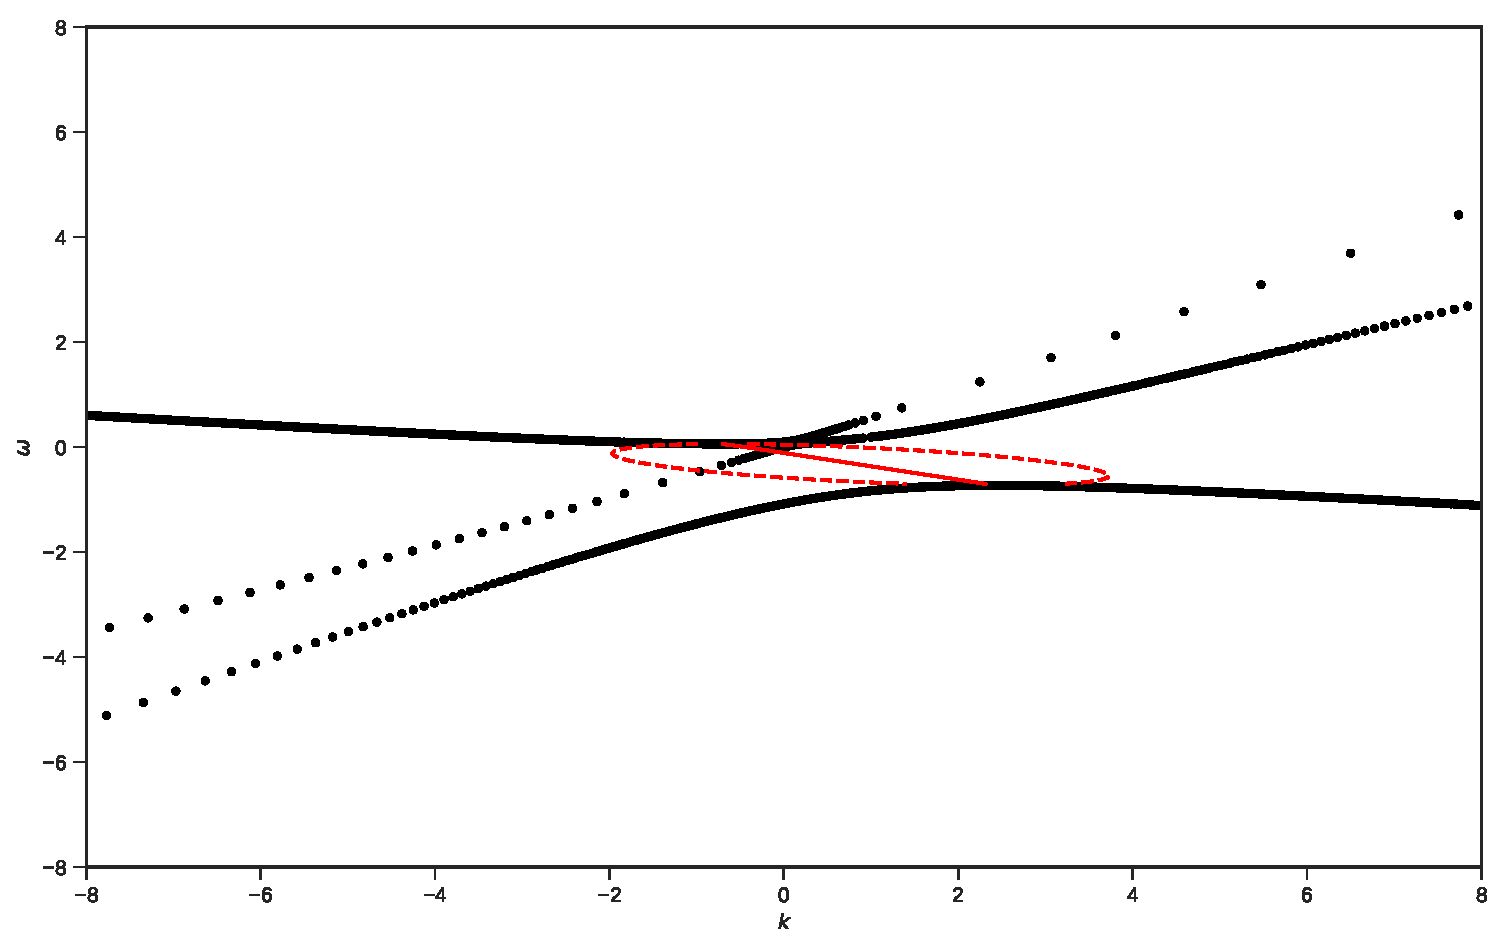
\includegraphics[width=\linewidth]{assets/spectDB3WC4DRDBMZAPltBlob.pdf}
\endminipage\hfill
\caption{Dispersion relation and instabilities of two zenith angles spectrum (upper panels) and three zenith angles spectrum (lower panels). The black lines are the dispersion relations and the colored dots are examples of complex $\omega$ for real $k$. The left panels are the dispersion relation and linear stability analysis of MAA solutions while the right panels are for MZA solutions.}
\label{fig-dr-db}
\end{figure}


However, this conclusion can not be generalized to arbitrary number of emission angles. As an example, we perform linear stability analysis of the three zenith angles emission configuration which is determined by a cubic function both in $\omega$ and $k$. Three solutions of $k(\omega)$ for given real $\omega(k)$  are expected. As long as real solutions disappear, complex solutions emerge, which leads to instabilities occur even without an actual gap. Rather the decrease in the number of real solutions for fixed $\omega$ or $k$ corresponds to the instabilities. In Fig. \ref{fig-dr-db}, we fix $\omega= 0.5$ for MAA solution (Fig. \ref{fig-dr-db} lower left panel). The three solutions of $k$ are $k=-4.6, 0.29, 1.2$.  $0.2$ which are all real and indicates no spatial instabilities. However, for another real $\omega = 0.2$, we find only one real solution $k=0.4$ from dispersion relation. The other solutions are complex and proven to be $k = -0.557106\pm 0.966535\mathrm i$ where the value with positive imaginary part leads to exponential growth. This gap and instability inconsistency also exists in continuous angular distribution of neutrino emission.



In core collapse supernova, neutrino emission is not in discrete zenith angles. More realistic models involves continuous zenith angle ELN spectra. In the earlier works of fast modes, Sawyer analyzed a box shaped angular distribution of neutrino emission \cite{Sawyer2016}. To address the fact that instability does not always show up in dispersion relation as gap, we show that the relation between instability and gap in dispersion relation can break down for box spectrum with crossing.



We construct a box spectrum with value $-0.1$ within $u\in [-1,-0.3)$ and value $1$ within $[-0.3,1]$ as shown in the top left panel of Fig. \ref{fig-box-c1}. With the spectrum defined, we calculate the dispersion relation and find out complex values of $k$ for real $\omega$. The results show that both the MAA solution and MZA solutioins contain only one curve. No gap is formed but we observe instabilities, which are plotted as colored dots.


\begin{figure}
   % \minipage{0.49\textwidth}
   %   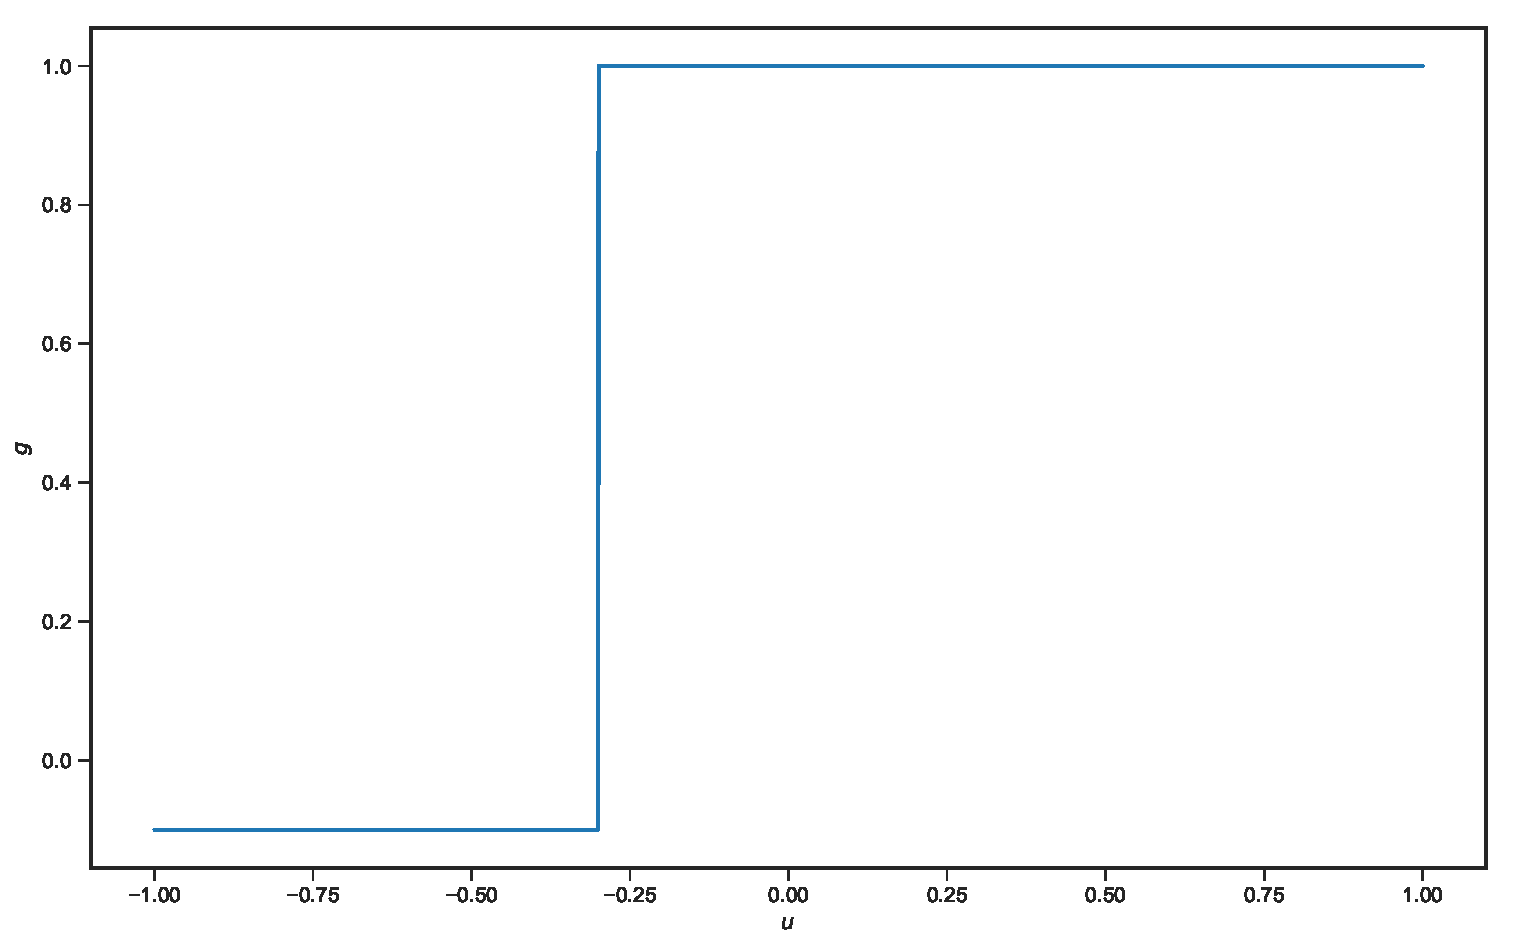
\includegraphics[width=\linewidth]{assets/spectBoxC1Spectrum.pdf}
   % \endminipage\hfill
   \minipage{0.49\textwidth}
   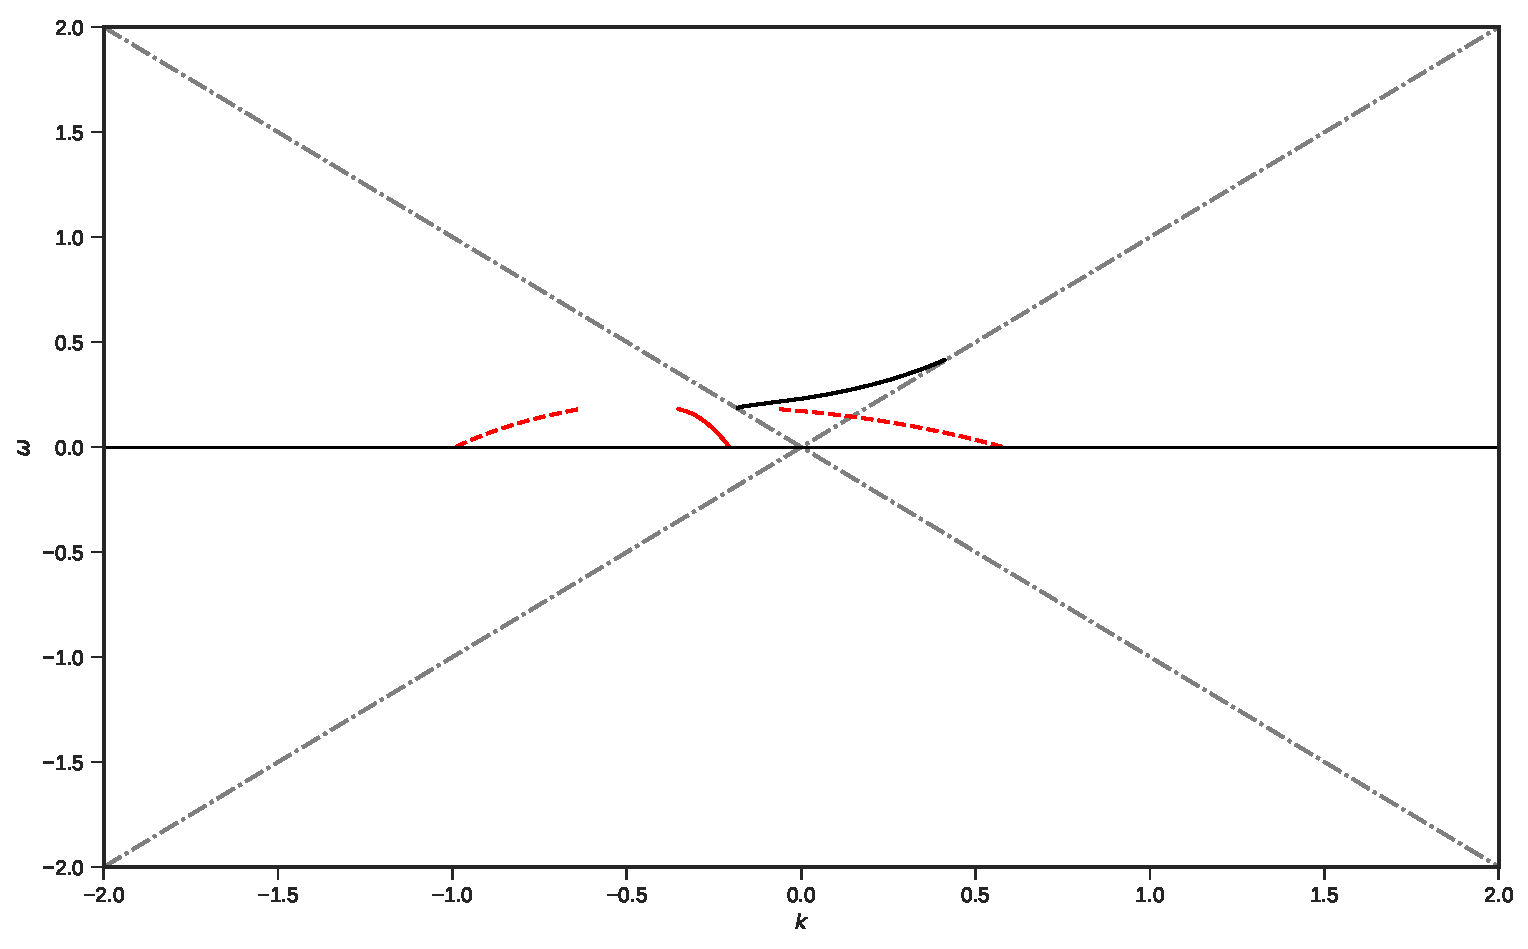
\includegraphics[width=\linewidth]{assets/spectBoxC1MAADRPltBlob.pdf}
   \endminipage\hfill
   \minipage{0.49\textwidth}
   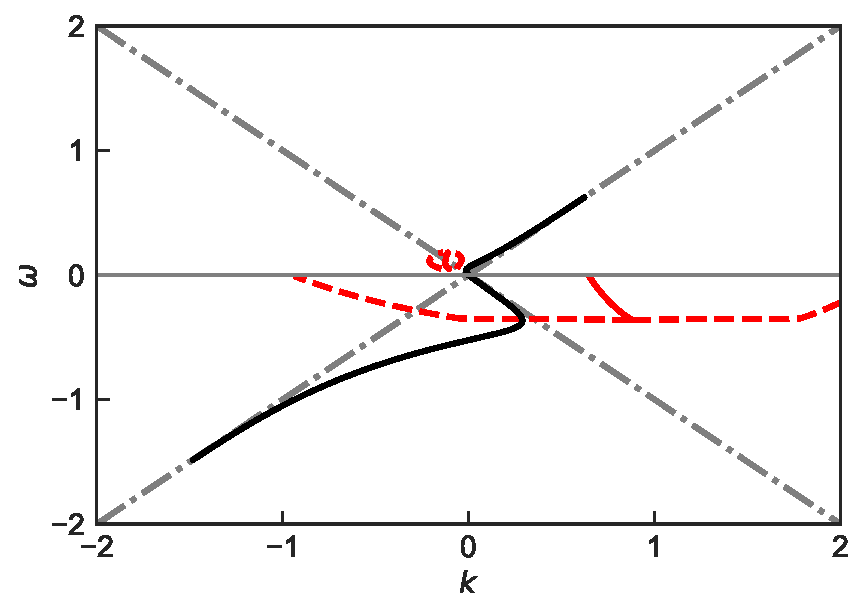
\includegraphics[width=\linewidth]{assets/spectBoxC1MZADRPltBlob.pdf}
   \endminipage\hfill
   \caption{Dispersion relation and linear stability analysis for box spectrum. The box spectrum is defined to be $-0.1$ within range $u\in [-1,-0.3)$ and $1$ within range $u\in [-0.3,1]$ as shown in the top left panel. The top right panel shows the dispersion relation and the complex $k$ for real $\omega$ for MAA solution. The lower panels shows the dispersion relation and complex $k$ for real $\omega$ for MZA solutions. Dashed gray lines are lines of $\omega= \pm k$ which sets the boundaries of the forbidden region for dispersion relation.
    }
   \label{fig-box-c1}
\end{figure}







{\color{red}\bf The forbidden region is determined by the emission angles. But is the forbidden region worth mentioning here? I don't think so.}

{\color{red}\bf I could show the results for C4 since it has both MAA and MZA instabilities. But we care about complex $k$ the most so I guess WC4 is fine.}

{\color{red}\bf Should I combine the MZA+ and MZA- solutions? }

{\color{red}\bf Font size in the plots are too small. But the font size depends on whether I need to combine MZA+ and MZA- solutions. }

{\color{red}\bf $\omega=0$ lines in the plots should be made distinguishable from the DR. }



\section{\label{sec-gap-to-instability}From Gap to Instability}

In the situations that the ELN spectrum has no crossing, gap indeed indicates instabilities, as shown in \onlinecite{Izaguirre2016a}. In this section we prove that the instabilities in MAA, MZA+, or MZA- solution can only appear in either region $\omega\leq 0$ or region $\omega \geq 0$. As it suggests, the instability regions propagate only between the dispersion relation and the axis $\omega=0$. We reproduce the calculation in \onlinecite{Izaguirre2016a} using the same Garching core-collapse supernova data set \cite{garching-ccsn-data}. The spectrum shown in the left panel of Fig. \ref{fig-garching} is polynomial fitting of the Garching 1D supernova simulation data.






\begin{figure}
   \minipage{0.49\textwidth}
     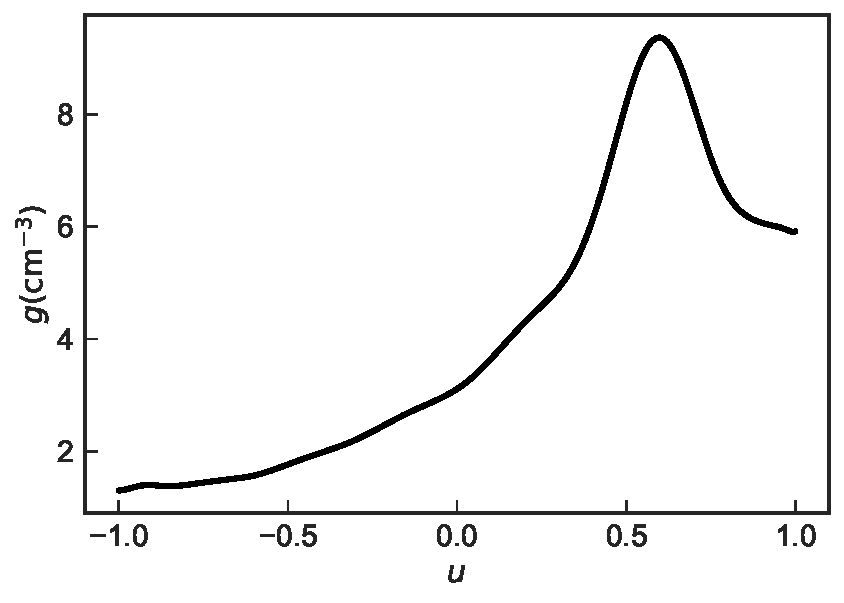
\includegraphics[width=\linewidth]{assets/spectGarchingPlt.pdf}
   \endminipage\hfill
   \minipage{0.49\textwidth}
   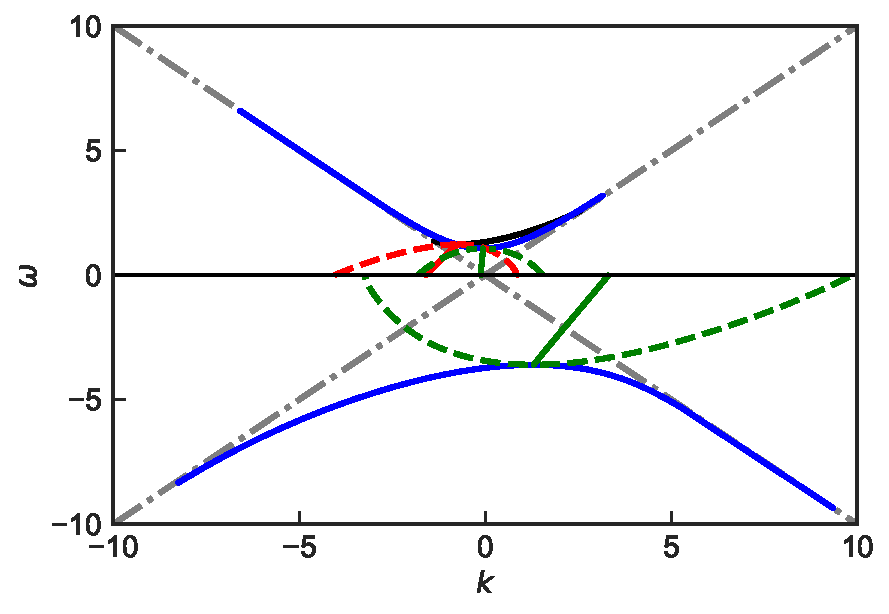
\includegraphics[width=\linewidth]{assets/spectGarchingDRLSAPltBlob.pdf}
   \endminipage\hfill
   \caption{Dispersion relation and linear stability analysis for a spectrum constructed from Garching 1D simulation data (left panel). From left to right, the sets of colored dots are the complex $k$ for MAA solution, MZA-, and MZA+ solutions respectively.
    }
   \label{fig-garching}
\end{figure}

{\color{red} \bf I haven't put in the correct unit for omega and k yet!!!! Remake the plots with the correct unit}


% \subsection{\label{sec-omega-to-zero}Instabilities at $\omega\to 0$}

For MAA solution of arbitrary spectrum, we write down the general form as
\begin{equation}
   4 = \bar I_0 - \bar I_2,
\end{equation}
where the $I_m$ is defined in the preceeding sections. Explicitly, we have to solve the integral function to find out $k$ for real $\omega$,
\begin{equation}
   k = \frac{1}{4} \int G(u) \frac{ 1 - u^2 }{ \omega/k - u }.
\end{equation}
For complex $k$, the integral can be decomposed into the principal value $\operatorname{Re}(k)$ and imaginary part $\operatorname{Im}(k)$ using Sokhotski–Plemelj theorem,
\begin{align}
\operatorname{Re}(k) =& \frac{1}{4}\left(  \mathcal{P} \int G(u) \frac{ 1 - u^2 }{  - u }  \right)\label{eqn-re-k-arbitrary-spectrum} \\
\operatorname{Im}(k) =&  \frac{\pi}{4}G(0) \operatorname{Sign}\left( \omega \right) \operatorname{Sign}\left(  \operatorname{Im}(k)  \right).
\label{eqn-im-k-arbitrary-spectrum}
\end{align}
We conclude from Eq. \eqref{eqn-im-k-arbitrary-spectrum} that $\omega$ has to have the same sign as $G(0)$. What's more, the value of $k$ at limit $\omega\to 0$ can be solved out of Eq. \eqref{eqn-re-k-arbitrary-spectrum} and Eq. \eqref{eqn-im-k-arbitrary-spectrum}. For instabilities the imaginary part of $k$ tells us the growth,
\begin{equation}
   \lvert \operatorname{Im}(k) \rvert  =  \frac{\pi}{4}\lvert G(0)\rvert .
\end{equation}
Similar result is obtained for MZA solutions,
\begin{align}
&\left(4\operatorname{Re}(k) - \mathcal P \int \frac{G(u)}{u} \mathrm d u + U_1 \right)^2  - \left( \operatorname{Sign}(\omega \operatorname{Im}(k) )\pi G(0) +4 \operatorname{Im}(k) \right)^2 \\
=&\left( \mathcal P \int \frac{G(u)}{u} \mathrm d u + U_1 \right)^2 -1 - 4 U_0^2  \\
&\left( 4 \operatorname{Re}(k) - \mathcal P \int \frac{G(u)}{u} \mathrm d u + U_1 \right) \left( \pi \operatorname{Sign}(\omega \operatorname{Im}(k) ) G(0) + 4 \operatorname{Im}(k) \right) \\
=& - \left( \mathcal P \int \frac{G(u)}{u} \mathrm du + U_1 \right) \pi \operatorname{Sign}(\omega \operatorname{Im}(k) ) G(0),
\end{align}
where $U_m = \int G(u) u^m \mathrm du$ and all the integrals are from $-1$ to $1$. The equations are quadratic in both $\operatorname{Re}(k)$ and $\operatorname{Im}(k)$ so the real solutions can be calculated and verified with linear stability analysis. The imaginary part $\operatorname{Im}(k)$
\begin{equation}
   \operatorname{Im}(k) = - \frac{1}{4} \pi G(0) \operatorname{Sign}(\omega k_I) \left(  1 + \frac{ \mathscr P \int \frac{G(u)}{u} du + \int G(u) u du }{ 4 \operatorname{Re}(k) - \mathscr P \int \frac{G(u)}{u} du + \int G(u) u du }  \right)
\end{equation}
determines that the two solutions are either in the region $\omega>0$ or in the region $\omega<0$ which corresponds to MZA+ and MZA- solutions.



\section{\label{sec-conclusion}Conclusion}




















%%%%%%%%%%%%%%%%%%%%%%%%%%%%%%%%%%%%%%%%%%%%%
%% APPENDIX
%%%%%%%%%%%%%%%%%%%%%%%%%%%%%%%%%%%%%%%%%%%%%

\appendix
\section{\label{sec-outline}Plan of the paper}



\begin{itemize}
    \item \sout{Review fast mode oscillations}
    \item \sout{State what has been done in Raffelt's paper.}
    \item \sout{The conclusion is not true.}
    \item \sout{Two zenith angles examples to prove that the number of solutions is the key.}
    \item \sout{Three zenith angles examples to show that not exactly related to gap.}
    \item Show that the continuous case is not related to gap at all. Box spectrum?
    \item Continuous spectrum or Garching group, data to show that we can prove the location of the instability.
    \item {\color{red}\bf Tweak the font size of plots.}
\end{itemize}



We are still not crystal clear about the relation between gap and lsa.





\bibliographystyle{apsrev4-1}
\bibliography{ref.bib}

\end{document}
%
% ****** End of file apssamp.tex ******
